% Options for packages loaded elsewhere
\PassOptionsToPackage{unicode}{hyperref}
\PassOptionsToPackage{hyphens}{url}
\PassOptionsToPackage{dvipsnames,svgnames,x11names}{xcolor}
%
\documentclass[
  letterpaper,
  DIV=11,
  numbers=noendperiod]{scrartcl}

\usepackage{amsmath,amssymb}
\usepackage{lmodern}
\usepackage{iftex}
\ifPDFTeX
  \usepackage[T1]{fontenc}
  \usepackage[utf8]{inputenc}
  \usepackage{textcomp} % provide euro and other symbols
\else % if luatex or xetex
  \usepackage{unicode-math}
  \defaultfontfeatures{Scale=MatchLowercase}
  \defaultfontfeatures[\rmfamily]{Ligatures=TeX,Scale=1}
\fi
% Use upquote if available, for straight quotes in verbatim environments
\IfFileExists{upquote.sty}{\usepackage{upquote}}{}
\IfFileExists{microtype.sty}{% use microtype if available
  \usepackage[]{microtype}
  \UseMicrotypeSet[protrusion]{basicmath} % disable protrusion for tt fonts
}{}
\makeatletter
\@ifundefined{KOMAClassName}{% if non-KOMA class
  \IfFileExists{parskip.sty}{%
    \usepackage{parskip}
  }{% else
    \setlength{\parindent}{0pt}
    \setlength{\parskip}{6pt plus 2pt minus 1pt}}
}{% if KOMA class
  \KOMAoptions{parskip=half}}
\makeatother
\usepackage{xcolor}
\setlength{\emergencystretch}{3em} % prevent overfull lines
\setcounter{secnumdepth}{-\maxdimen} % remove section numbering
% Make \paragraph and \subparagraph free-standing
\ifx\paragraph\undefined\else
  \let\oldparagraph\paragraph
  \renewcommand{\paragraph}[1]{\oldparagraph{#1}\mbox{}}
\fi
\ifx\subparagraph\undefined\else
  \let\oldsubparagraph\subparagraph
  \renewcommand{\subparagraph}[1]{\oldsubparagraph{#1}\mbox{}}
\fi

\usepackage{color}
\usepackage{fancyvrb}
\newcommand{\VerbBar}{|}
\newcommand{\VERB}{\Verb[commandchars=\\\{\}]}
\DefineVerbatimEnvironment{Highlighting}{Verbatim}{commandchars=\\\{\}}
% Add ',fontsize=\small' for more characters per line
\usepackage{framed}
\definecolor{shadecolor}{RGB}{241,243,245}
\newenvironment{Shaded}{\begin{snugshade}}{\end{snugshade}}
\newcommand{\AlertTok}[1]{\textcolor[rgb]{0.68,0.00,0.00}{#1}}
\newcommand{\AnnotationTok}[1]{\textcolor[rgb]{0.37,0.37,0.37}{#1}}
\newcommand{\AttributeTok}[1]{\textcolor[rgb]{0.40,0.45,0.13}{#1}}
\newcommand{\BaseNTok}[1]{\textcolor[rgb]{0.68,0.00,0.00}{#1}}
\newcommand{\BuiltInTok}[1]{\textcolor[rgb]{0.00,0.23,0.31}{#1}}
\newcommand{\CharTok}[1]{\textcolor[rgb]{0.13,0.47,0.30}{#1}}
\newcommand{\CommentTok}[1]{\textcolor[rgb]{0.37,0.37,0.37}{#1}}
\newcommand{\CommentVarTok}[1]{\textcolor[rgb]{0.37,0.37,0.37}{\textit{#1}}}
\newcommand{\ConstantTok}[1]{\textcolor[rgb]{0.56,0.35,0.01}{#1}}
\newcommand{\ControlFlowTok}[1]{\textcolor[rgb]{0.00,0.23,0.31}{#1}}
\newcommand{\DataTypeTok}[1]{\textcolor[rgb]{0.68,0.00,0.00}{#1}}
\newcommand{\DecValTok}[1]{\textcolor[rgb]{0.68,0.00,0.00}{#1}}
\newcommand{\DocumentationTok}[1]{\textcolor[rgb]{0.37,0.37,0.37}{\textit{#1}}}
\newcommand{\ErrorTok}[1]{\textcolor[rgb]{0.68,0.00,0.00}{#1}}
\newcommand{\ExtensionTok}[1]{\textcolor[rgb]{0.00,0.23,0.31}{#1}}
\newcommand{\FloatTok}[1]{\textcolor[rgb]{0.68,0.00,0.00}{#1}}
\newcommand{\FunctionTok}[1]{\textcolor[rgb]{0.28,0.35,0.67}{#1}}
\newcommand{\ImportTok}[1]{\textcolor[rgb]{0.00,0.46,0.62}{#1}}
\newcommand{\InformationTok}[1]{\textcolor[rgb]{0.37,0.37,0.37}{#1}}
\newcommand{\KeywordTok}[1]{\textcolor[rgb]{0.00,0.23,0.31}{#1}}
\newcommand{\NormalTok}[1]{\textcolor[rgb]{0.00,0.23,0.31}{#1}}
\newcommand{\OperatorTok}[1]{\textcolor[rgb]{0.37,0.37,0.37}{#1}}
\newcommand{\OtherTok}[1]{\textcolor[rgb]{0.00,0.23,0.31}{#1}}
\newcommand{\PreprocessorTok}[1]{\textcolor[rgb]{0.68,0.00,0.00}{#1}}
\newcommand{\RegionMarkerTok}[1]{\textcolor[rgb]{0.00,0.23,0.31}{#1}}
\newcommand{\SpecialCharTok}[1]{\textcolor[rgb]{0.37,0.37,0.37}{#1}}
\newcommand{\SpecialStringTok}[1]{\textcolor[rgb]{0.13,0.47,0.30}{#1}}
\newcommand{\StringTok}[1]{\textcolor[rgb]{0.13,0.47,0.30}{#1}}
\newcommand{\VariableTok}[1]{\textcolor[rgb]{0.07,0.07,0.07}{#1}}
\newcommand{\VerbatimStringTok}[1]{\textcolor[rgb]{0.13,0.47,0.30}{#1}}
\newcommand{\WarningTok}[1]{\textcolor[rgb]{0.37,0.37,0.37}{\textit{#1}}}

\providecommand{\tightlist}{%
  \setlength{\itemsep}{0pt}\setlength{\parskip}{0pt}}\usepackage{longtable,booktabs,array}
\usepackage{calc} % for calculating minipage widths
% Correct order of tables after \paragraph or \subparagraph
\usepackage{etoolbox}
\makeatletter
\patchcmd\longtable{\par}{\if@noskipsec\mbox{}\fi\par}{}{}
\makeatother
% Allow footnotes in longtable head/foot
\IfFileExists{footnotehyper.sty}{\usepackage{footnotehyper}}{\usepackage{footnote}}
\makesavenoteenv{longtable}
\usepackage{graphicx}
\makeatletter
\def\maxwidth{\ifdim\Gin@nat@width>\linewidth\linewidth\else\Gin@nat@width\fi}
\def\maxheight{\ifdim\Gin@nat@height>\textheight\textheight\else\Gin@nat@height\fi}
\makeatother
% Scale images if necessary, so that they will not overflow the page
% margins by default, and it is still possible to overwrite the defaults
% using explicit options in \includegraphics[width, height, ...]{}
\setkeys{Gin}{width=\maxwidth,height=\maxheight,keepaspectratio}
% Set default figure placement to htbp
\makeatletter
\def\fps@figure{htbp}
\makeatother

\KOMAoption{captions}{tableheading}
\makeatletter
\makeatother
\makeatletter
\makeatother
\makeatletter
\@ifpackageloaded{caption}{}{\usepackage{caption}}
\AtBeginDocument{%
\ifdefined\contentsname
  \renewcommand*\contentsname{Table of contents}
\else
  \newcommand\contentsname{Table of contents}
\fi
\ifdefined\listfigurename
  \renewcommand*\listfigurename{List of Figures}
\else
  \newcommand\listfigurename{List of Figures}
\fi
\ifdefined\listtablename
  \renewcommand*\listtablename{List of Tables}
\else
  \newcommand\listtablename{List of Tables}
\fi
\ifdefined\figurename
  \renewcommand*\figurename{Figure}
\else
  \newcommand\figurename{Figure}
\fi
\ifdefined\tablename
  \renewcommand*\tablename{Table}
\else
  \newcommand\tablename{Table}
\fi
}
\@ifpackageloaded{float}{}{\usepackage{float}}
\floatstyle{ruled}
\@ifundefined{c@chapter}{\newfloat{codelisting}{h}{lop}}{\newfloat{codelisting}{h}{lop}[chapter]}
\floatname{codelisting}{Listing}
\newcommand*\listoflistings{\listof{codelisting}{List of Listings}}
\makeatother
\makeatletter
\@ifpackageloaded{caption}{}{\usepackage{caption}}
\@ifpackageloaded{subcaption}{}{\usepackage{subcaption}}
\makeatother
\makeatletter
\@ifpackageloaded{tcolorbox}{}{\usepackage[many]{tcolorbox}}
\makeatother
\makeatletter
\@ifundefined{shadecolor}{\definecolor{shadecolor}{rgb}{.97, .97, .97}}
\makeatother
\makeatletter
\makeatother
\ifLuaTeX
  \usepackage{selnolig}  % disable illegal ligatures
\fi
\IfFileExists{bookmark.sty}{\usepackage{bookmark}}{\usepackage{hyperref}}
\IfFileExists{xurl.sty}{\usepackage{xurl}}{} % add URL line breaks if available
\urlstyle{same} % disable monospaced font for URLs
\hypersetup{
  pdftitle={Class 12: RNASeq analysis},
  pdfauthor={Eric Jordahl},
  colorlinks=true,
  linkcolor={blue},
  filecolor={Maroon},
  citecolor={Blue},
  urlcolor={Blue},
  pdfcreator={LaTeX via pandoc}}

\title{Class 12: RNASeq analysis}
\author{Eric Jordahl}
\date{2022-11-4}

\begin{document}
\maketitle
\ifdefined\Shaded\renewenvironment{Shaded}{\begin{tcolorbox}[frame hidden, boxrule=0pt, enhanced, breakable, borderline west={3pt}{0pt}{shadecolor}, interior hidden, sharp corners]}{\end{tcolorbox}}\fi

\renewcommand*\contentsname{Table of contents}
{
\hypersetup{linkcolor=}
\setcounter{tocdepth}{3}
\tableofcontents
}
\hypertarget{transcriptomics}{%
\section{Transcriptomics}\label{transcriptomics}}

\hypertarget{import-countdata-and-coldata}{%
\subsection{Import CountData and
ColData}\label{import-countdata-and-coldata}}

\begin{Shaded}
\begin{Highlighting}[]
\FunctionTok{library}\NormalTok{(BiocManager)}
\FunctionTok{library}\NormalTok{(DESeq2)}
\end{Highlighting}
\end{Shaded}

\begin{Shaded}
\begin{Highlighting}[]
\NormalTok{counts }\OtherTok{\textless{}{-}} \FunctionTok{read.csv}\NormalTok{(}\StringTok{"airway\_scaledcounts.csv"}\NormalTok{, }\AttributeTok{row.names=}\DecValTok{1}\NormalTok{)}
\NormalTok{metadata }\OtherTok{\textless{}{-}}  \FunctionTok{read.csv}\NormalTok{(}\StringTok{"airway\_metadata.csv"}\NormalTok{)}
\end{Highlighting}
\end{Shaded}

\begin{Shaded}
\begin{Highlighting}[]
\FunctionTok{head}\NormalTok{(counts)}
\end{Highlighting}
\end{Shaded}

\begin{verbatim}
                SRR1039508 SRR1039509 SRR1039512 SRR1039513 SRR1039516
ENSG00000000003        723        486        904        445       1170
ENSG00000000005          0          0          0          0          0
ENSG00000000419        467        523        616        371        582
ENSG00000000457        347        258        364        237        318
ENSG00000000460         96         81         73         66        118
ENSG00000000938          0          0          1          0          2
                SRR1039517 SRR1039520 SRR1039521
ENSG00000000003       1097        806        604
ENSG00000000005          0          0          0
ENSG00000000419        781        417        509
ENSG00000000457        447        330        324
ENSG00000000460         94        102         74
ENSG00000000938          0          0          0
\end{verbatim}

\begin{Shaded}
\begin{Highlighting}[]
\FunctionTok{head}\NormalTok{(metadata)}
\end{Highlighting}
\end{Shaded}

\begin{verbatim}
          id     dex celltype     geo_id
1 SRR1039508 control   N61311 GSM1275862
2 SRR1039509 treated   N61311 GSM1275863
3 SRR1039512 control  N052611 GSM1275866
4 SRR1039513 treated  N052611 GSM1275867
5 SRR1039516 control  N080611 GSM1275870
6 SRR1039517 treated  N080611 GSM1275871
\end{verbatim}

\hypertarget{q1}{%
\subsection{\texorpdfstring{\textbf{Q1}}{Q1}}\label{q1}}

\textbf{How many genes are in this dataset?}

\begin{Shaded}
\begin{Highlighting}[]
\FunctionTok{nrow}\NormalTok{(counts)}
\end{Highlighting}
\end{Shaded}

\begin{verbatim}
[1] 38694
\end{verbatim}

There are 38694 genes in this dataset

\hypertarget{q2}{%
\subsection{\texorpdfstring{\textbf{Q2}}{Q2}}\label{q2}}

\textbf{How many `control' cell lines do we have?}

\begin{Shaded}
\begin{Highlighting}[]
\FunctionTok{table}\NormalTok{(metadata}\SpecialCharTok{$}\NormalTok{dex)}
\end{Highlighting}
\end{Shaded}

\begin{verbatim}

control treated 
      4       4 
\end{verbatim}

There are 4 control cell lines in thsi dataset

\hypertarget{toy-differential-gene-expression}{%
\section{Toy Differential Gene
Expression}\label{toy-differential-gene-expression}}

\begin{Shaded}
\begin{Highlighting}[]
\NormalTok{control }\OtherTok{\textless{}{-}}\NormalTok{ metadata[metadata[,}\StringTok{"dex"}\NormalTok{]}\SpecialCharTok{==}\StringTok{"control"}\NormalTok{,]}
\NormalTok{control.counts }\OtherTok{\textless{}{-}}\NormalTok{ counts[ ,control}\SpecialCharTok{$}\NormalTok{id]}
\NormalTok{control.mean }\OtherTok{\textless{}{-}} \FunctionTok{rowSums}\NormalTok{( control.counts )}\SpecialCharTok{/}\DecValTok{4} 
\FunctionTok{head}\NormalTok{(control.mean)}
\end{Highlighting}
\end{Shaded}

\begin{verbatim}
ENSG00000000003 ENSG00000000005 ENSG00000000419 ENSG00000000457 ENSG00000000460 
         900.75            0.00          520.50          339.75           97.25 
ENSG00000000938 
           0.75 
\end{verbatim}

\begin{Shaded}
\begin{Highlighting}[]
\FunctionTok{library}\NormalTok{(dplyr)}
\NormalTok{control }\OtherTok{\textless{}{-}}\NormalTok{ metadata }\SpecialCharTok{\%\textgreater{}\%} \FunctionTok{filter}\NormalTok{(dex}\SpecialCharTok{==}\StringTok{"control"}\NormalTok{)}
\NormalTok{control.counts }\OtherTok{\textless{}{-}}\NormalTok{ counts }\SpecialCharTok{\%\textgreater{}\%} \FunctionTok{select}\NormalTok{(control}\SpecialCharTok{$}\NormalTok{id) }
\NormalTok{control.mean }\OtherTok{\textless{}{-}} \FunctionTok{rowSums}\NormalTok{(control.counts)}\SpecialCharTok{/}\DecValTok{4}
\FunctionTok{head}\NormalTok{(control.mean)}
\end{Highlighting}
\end{Shaded}

\begin{verbatim}
ENSG00000000003 ENSG00000000005 ENSG00000000419 ENSG00000000457 ENSG00000000460 
         900.75            0.00          520.50          339.75           97.25 
ENSG00000000938 
           0.75 
\end{verbatim}

\hypertarget{q3}{%
\subsection{\texorpdfstring{\textbf{Q3}}{Q3}}\label{q3}}

\textbf{How would you make the above code in either approach more
robust?}

You could make this code more robust my making it a function so that you
can just plug in either control or treated and get the mean for both
without having to go through the code twice

\hypertarget{q4}{%
\subsection{\texorpdfstring{\textbf{Q4}}{Q4}}\label{q4}}

\textbf{Follow the same procedure for the treated samples
(i.e.~calculate the mean per gene across drug treated samples and assign
to a labeled vector called treated.mean)}

\begin{Shaded}
\begin{Highlighting}[]
\NormalTok{treated }\OtherTok{\textless{}{-}}\NormalTok{ metadata[metadata[,}\StringTok{"dex"}\NormalTok{]}\SpecialCharTok{==}\StringTok{"treated"}\NormalTok{,]}
\NormalTok{treated.counts }\OtherTok{\textless{}{-}}\NormalTok{ counts[ ,treated}\SpecialCharTok{$}\NormalTok{id]}
\NormalTok{treated.mean }\OtherTok{\textless{}{-}} \FunctionTok{rowSums}\NormalTok{( treated.counts )}\SpecialCharTok{/}\DecValTok{4} 
\FunctionTok{head}\NormalTok{(treated.mean)}
\end{Highlighting}
\end{Shaded}

\begin{verbatim}
ENSG00000000003 ENSG00000000005 ENSG00000000419 ENSG00000000457 ENSG00000000460 
         658.00            0.00          546.00          316.50           78.75 
ENSG00000000938 
           0.00 
\end{verbatim}

\begin{Shaded}
\begin{Highlighting}[]
\NormalTok{meancounts }\OtherTok{\textless{}{-}} \FunctionTok{data.frame}\NormalTok{(control.mean, treated.mean)}
\end{Highlighting}
\end{Shaded}

\hypertarget{q5-a}{%
\subsection{\texorpdfstring{\textbf{Q5 (a)}}{Q5 (a)}}\label{q5-a}}

\textbf{Create a scatter plot showing the mean of the treated samples
against the mean of the control samples}

\begin{Shaded}
\begin{Highlighting}[]
\FunctionTok{plot}\NormalTok{(meancounts)}
\end{Highlighting}
\end{Shaded}

\begin{figure}[H]

{\centering 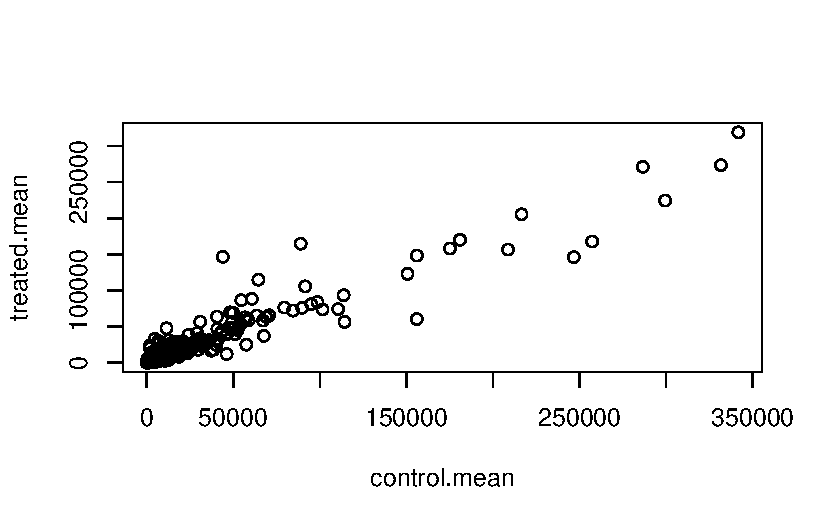
\includegraphics{Class12_files/figure-pdf/unnamed-chunk-10-1.pdf}

}

\end{figure}

\hypertarget{q5-b}{%
\subsection{\texorpdfstring{\textbf{Q5 (b)}}{Q5 (b)}}\label{q5-b}}

\textbf{You could also use the ggplot2 package to make this figure
producing the plot below. What geom\_?() function would you use for this
plot?}

I could also use the geom\_point() function to plot this using ggplot2

\hypertarget{q6}{%
\subsection{\texorpdfstring{\textbf{Q6}}{Q6}}\label{q6}}

\textbf{Try plotting both axes on a log scale. What is the argument to
plot() that allows you to do this?}

\begin{Shaded}
\begin{Highlighting}[]
\FunctionTok{plot}\NormalTok{(meancounts, }\AttributeTok{log=}\StringTok{"xy"}\NormalTok{)}
\end{Highlighting}
\end{Shaded}

\begin{verbatim}
Warning in xy.coords(x, y, xlabel, ylabel, log): 15032 x values <= 0 omitted
from logarithmic plot
\end{verbatim}

\begin{verbatim}
Warning in xy.coords(x, y, xlabel, ylabel, log): 15281 y values <= 0 omitted
from logarithmic plot
\end{verbatim}

\begin{figure}[H]

{\centering 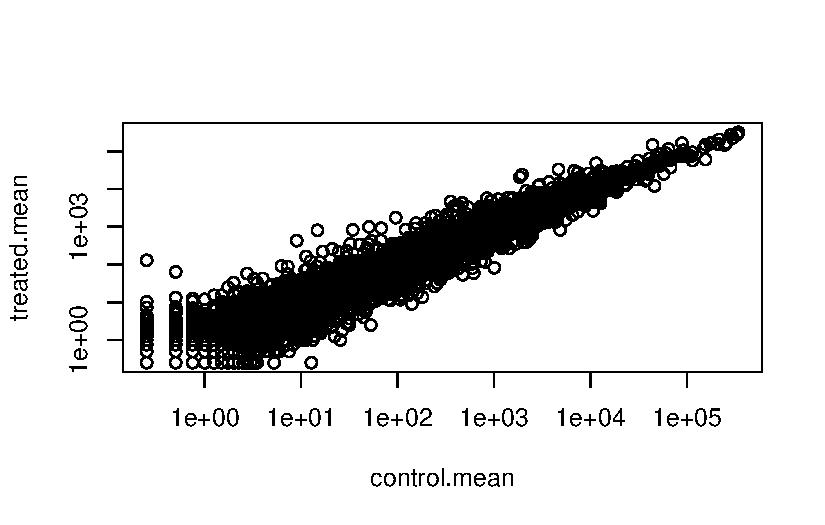
\includegraphics{Class12_files/figure-pdf/unnamed-chunk-11-1.pdf}

}

\end{figure}

You can use the ``log'' setting in the default plot, to set x and y
scale to logarithmic

\begin{Shaded}
\begin{Highlighting}[]
\NormalTok{meancounts}\SpecialCharTok{$}\NormalTok{log2fc }\OtherTok{\textless{}{-}} \FunctionTok{log2}\NormalTok{(meancounts[,}\StringTok{"treated.mean"}\NormalTok{]}\SpecialCharTok{/}\NormalTok{meancounts[,}\StringTok{"control.mean"}\NormalTok{])}
\FunctionTok{head}\NormalTok{(meancounts)}
\end{Highlighting}
\end{Shaded}

\begin{verbatim}
                control.mean treated.mean      log2fc
ENSG00000000003       900.75       658.00 -0.45303916
ENSG00000000005         0.00         0.00         NaN
ENSG00000000419       520.50       546.00  0.06900279
ENSG00000000457       339.75       316.50 -0.10226805
ENSG00000000460        97.25        78.75 -0.30441833
ENSG00000000938         0.75         0.00        -Inf
\end{verbatim}

\begin{Shaded}
\begin{Highlighting}[]
\NormalTok{zero.vals }\OtherTok{\textless{}{-}} \FunctionTok{which}\NormalTok{(meancounts[,}\DecValTok{1}\SpecialCharTok{:}\DecValTok{2}\NormalTok{]}\SpecialCharTok{==}\DecValTok{0}\NormalTok{, }\AttributeTok{arr.ind=}\ConstantTok{TRUE}\NormalTok{)}
\NormalTok{to.rm }\OtherTok{\textless{}{-}} \FunctionTok{unique}\NormalTok{(zero.vals[,}\DecValTok{1}\NormalTok{])}
\NormalTok{mycounts }\OtherTok{\textless{}{-}}\NormalTok{ meancounts[}\SpecialCharTok{{-}}\NormalTok{to.rm,]}
\FunctionTok{nrow}\NormalTok{(mycounts)}
\end{Highlighting}
\end{Shaded}

\begin{verbatim}
[1] 21817
\end{verbatim}

\hypertarget{q7}{%
\subsection{\texorpdfstring{\textbf{Q7}}{Q7}}\label{q7}}

\textbf{What is the purpose of the arr.ind argument in the which()
function call above? Why would we then take the first column of the
output and need to call the unique() function?}

The arr.ind argument allows us to identify the entries that do not have
any measurements so that we can remove them from the dataset without
factoring them into the rest of the data.

\begin{Shaded}
\begin{Highlighting}[]
\NormalTok{up.ind }\OtherTok{\textless{}{-}}\NormalTok{ mycounts}\SpecialCharTok{$}\NormalTok{log2fc }\SpecialCharTok{\textgreater{}} \DecValTok{2}
\NormalTok{down.ind }\OtherTok{\textless{}{-}}\NormalTok{ mycounts}\SpecialCharTok{$}\NormalTok{log2fc }\SpecialCharTok{\textless{}}\NormalTok{ (}\SpecialCharTok{{-}}\DecValTok{2}\NormalTok{)}
\FunctionTok{sum}\NormalTok{(up.ind)}
\end{Highlighting}
\end{Shaded}

\begin{verbatim}
[1] 250
\end{verbatim}

\begin{Shaded}
\begin{Highlighting}[]
\FunctionTok{sum}\NormalTok{(down.ind)}
\end{Highlighting}
\end{Shaded}

\begin{verbatim}
[1] 367
\end{verbatim}

\hypertarget{q8}{%
\subsection{\texorpdfstring{\textbf{Q8}}{Q8}}\label{q8}}

\textbf{Using the up.ind vector above can you determine how many up
regulated genes we have at the greater than 2 fc level?}

There are 250 genes

\hypertarget{q9}{%
\subsection{\texorpdfstring{\textbf{Q9}}{Q9}}\label{q9}}

\textbf{Using the down.ind vector above can you determine how many down
regulated genes we have at the greater than 2 fc level?}

There are 367 genes

\hypertarget{q10}{%
\subsection{\texorpdfstring{\textbf{Q10}}{Q10}}\label{q10}}

\textbf{Do you trust these results? Why or why not?}

No, we do not have a statistical significance at this point, so we
cannot tell if this is imporant or not yet without running a T-Test.

\hypertarget{deseq2-analysis}{%
\section{DESeq2 analysis}\label{deseq2-analysis}}

\begin{Shaded}
\begin{Highlighting}[]
\FunctionTok{library}\NormalTok{(DESeq2)}
\FunctionTok{citation}\NormalTok{(}\StringTok{"DESeq2"}\NormalTok{)}
\end{Highlighting}
\end{Shaded}

\begin{verbatim}

To cite package 'DESeq2' in publications use:

  Love, M.I., Huber, W., Anders, S. Moderated estimation of fold change
  and dispersion for RNA-seq data with DESeq2 Genome Biology 15(12):550
  (2014)

A BibTeX entry for LaTeX users is

  @Article{,
    title = {Moderated estimation of fold change and dispersion for RNA-seq data with DESeq2},
    author = {Michael I. Love and Wolfgang Huber and Simon Anders},
    year = {2014},
    journal = {Genome Biology},
    doi = {10.1186/s13059-014-0550-8},
    volume = {15},
    issue = {12},
    pages = {550},
  }
\end{verbatim}

\begin{Shaded}
\begin{Highlighting}[]
\NormalTok{dds }\OtherTok{\textless{}{-}} \FunctionTok{DESeqDataSetFromMatrix}\NormalTok{(}\AttributeTok{countData=}\NormalTok{counts, }
                              \AttributeTok{colData=}\NormalTok{metadata, }
                              \AttributeTok{design=}\SpecialCharTok{\textasciitilde{}}\NormalTok{dex)}
\end{Highlighting}
\end{Shaded}

\begin{verbatim}
converting counts to integer mode
\end{verbatim}

\begin{verbatim}
Warning in DESeqDataSet(se, design = design, ignoreRank): some variables in
design formula are characters, converting to factors
\end{verbatim}

\begin{Shaded}
\begin{Highlighting}[]
\NormalTok{dds}
\end{Highlighting}
\end{Shaded}

\begin{verbatim}
class: DESeqDataSet 
dim: 38694 8 
metadata(1): version
assays(1): counts
rownames(38694): ENSG00000000003 ENSG00000000005 ... ENSG00000283120
  ENSG00000283123
rowData names(0):
colnames(8): SRR1039508 SRR1039509 ... SRR1039520 SRR1039521
colData names(4): id dex celltype geo_id
\end{verbatim}

\begin{Shaded}
\begin{Highlighting}[]
\NormalTok{dds }\OtherTok{\textless{}{-}} \FunctionTok{DESeq}\NormalTok{(dds)}
\NormalTok{res }\OtherTok{\textless{}{-}} \FunctionTok{results}\NormalTok{(dds)}
\NormalTok{res}
\end{Highlighting}
\end{Shaded}

\begin{verbatim}
log2 fold change (MLE): dex treated vs control 
Wald test p-value: dex treated vs control 
DataFrame with 38694 rows and 6 columns
                 baseMean log2FoldChange     lfcSE      stat    pvalue
                <numeric>      <numeric> <numeric> <numeric> <numeric>
ENSG00000000003  747.1942     -0.3507030  0.168246 -2.084470 0.0371175
ENSG00000000005    0.0000             NA        NA        NA        NA
ENSG00000000419  520.1342      0.2061078  0.101059  2.039475 0.0414026
ENSG00000000457  322.6648      0.0245269  0.145145  0.168982 0.8658106
ENSG00000000460   87.6826     -0.1471420  0.257007 -0.572521 0.5669691
...                   ...            ...       ...       ...       ...
ENSG00000283115  0.000000             NA        NA        NA        NA
ENSG00000283116  0.000000             NA        NA        NA        NA
ENSG00000283119  0.000000             NA        NA        NA        NA
ENSG00000283120  0.974916      -0.668258   1.69456 -0.394354  0.693319
ENSG00000283123  0.000000             NA        NA        NA        NA
                     padj
                <numeric>
ENSG00000000003  0.163035
ENSG00000000005        NA
ENSG00000000419  0.176032
ENSG00000000457  0.961694
ENSG00000000460  0.815849
...                   ...
ENSG00000283115        NA
ENSG00000283116        NA
ENSG00000283119        NA
ENSG00000283120        NA
ENSG00000283123        NA
\end{verbatim}

\begin{Shaded}
\begin{Highlighting}[]
\FunctionTok{summary}\NormalTok{(res)}
\end{Highlighting}
\end{Shaded}

\begin{verbatim}

out of 25258 with nonzero total read count
adjusted p-value < 0.1
LFC > 0 (up)       : 1563, 6.2%
LFC < 0 (down)     : 1188, 4.7%
outliers [1]       : 142, 0.56%
low counts [2]     : 9971, 39%
(mean count < 10)
[1] see 'cooksCutoff' argument of ?results
[2] see 'independentFiltering' argument of ?results
\end{verbatim}

\begin{Shaded}
\begin{Highlighting}[]
\NormalTok{res05 }\OtherTok{\textless{}{-}} \FunctionTok{results}\NormalTok{(dds, }\AttributeTok{alpha=}\FloatTok{0.05}\NormalTok{)}
\FunctionTok{summary}\NormalTok{(res05)}
\end{Highlighting}
\end{Shaded}

\begin{verbatim}

out of 25258 with nonzero total read count
adjusted p-value < 0.05
LFC > 0 (up)       : 1236, 4.9%
LFC < 0 (down)     : 933, 3.7%
outliers [1]       : 142, 0.56%
low counts [2]     : 9033, 36%
(mean count < 6)
[1] see 'cooksCutoff' argument of ?results
[2] see 'independentFiltering' argument of ?results
\end{verbatim}

\hypertarget{adding-annotation-data}{%
\section{Adding Annotation Data}\label{adding-annotation-data}}

\begin{Shaded}
\begin{Highlighting}[]
\FunctionTok{library}\NormalTok{(}\StringTok{"AnnotationDbi"}\NormalTok{)}
\end{Highlighting}
\end{Shaded}

\begin{verbatim}

Attaching package: 'AnnotationDbi'
\end{verbatim}

\begin{verbatim}
The following object is masked from 'package:dplyr':

    select
\end{verbatim}

\begin{Shaded}
\begin{Highlighting}[]
\FunctionTok{library}\NormalTok{(}\StringTok{"org.Hs.eg.db"}\NormalTok{)}
\end{Highlighting}
\end{Shaded}

\begin{verbatim}
\end{verbatim}

\begin{Shaded}
\begin{Highlighting}[]
\FunctionTok{columns}\NormalTok{(org.Hs.eg.db)}
\end{Highlighting}
\end{Shaded}

\begin{verbatim}
 [1] "ACCNUM"       "ALIAS"        "ENSEMBL"      "ENSEMBLPROT"  "ENSEMBLTRANS"
 [6] "ENTREZID"     "ENZYME"       "EVIDENCE"     "EVIDENCEALL"  "GENENAME"    
[11] "GENETYPE"     "GO"           "GOALL"        "IPI"          "MAP"         
[16] "OMIM"         "ONTOLOGY"     "ONTOLOGYALL"  "PATH"         "PFAM"        
[21] "PMID"         "PROSITE"      "REFSEQ"       "SYMBOL"       "UCSCKG"      
[26] "UNIPROT"     
\end{verbatim}

\begin{Shaded}
\begin{Highlighting}[]
\NormalTok{res}\SpecialCharTok{$}\NormalTok{symbol }\OtherTok{\textless{}{-}} \FunctionTok{mapIds}\NormalTok{(org.Hs.eg.db,}
                     \AttributeTok{keys=}\FunctionTok{row.names}\NormalTok{(res), }\CommentTok{\# Our genenames}
                     \AttributeTok{keytype=}\StringTok{"ENSEMBL"}\NormalTok{,        }\CommentTok{\# The format of our genenames}
                     \AttributeTok{column=}\StringTok{"SYMBOL"}\NormalTok{,          }\CommentTok{\# The new format we want to add}
                     \AttributeTok{multiVals=}\StringTok{"first"}\NormalTok{)}
\FunctionTok{head}\NormalTok{(res)}
\end{Highlighting}
\end{Shaded}

\begin{verbatim}
log2 fold change (MLE): dex treated vs control 
Wald test p-value: dex treated vs control 
DataFrame with 6 rows and 7 columns
                  baseMean log2FoldChange     lfcSE      stat    pvalue
                 <numeric>      <numeric> <numeric> <numeric> <numeric>
ENSG00000000003 747.194195     -0.3507030  0.168246 -2.084470 0.0371175
ENSG00000000005   0.000000             NA        NA        NA        NA
ENSG00000000419 520.134160      0.2061078  0.101059  2.039475 0.0414026
ENSG00000000457 322.664844      0.0245269  0.145145  0.168982 0.8658106
ENSG00000000460  87.682625     -0.1471420  0.257007 -0.572521 0.5669691
ENSG00000000938   0.319167     -1.7322890  3.493601 -0.495846 0.6200029
                     padj      symbol
                <numeric> <character>
ENSG00000000003  0.163035      TSPAN6
ENSG00000000005        NA        TNMD
ENSG00000000419  0.176032        DPM1
ENSG00000000457  0.961694       SCYL3
ENSG00000000460  0.815849    C1orf112
ENSG00000000938        NA         FGR
\end{verbatim}

\hypertarget{q11}{%
\subsection{\texorpdfstring{\textbf{Q11}}{Q11}}\label{q11}}

\textbf{Run the mapIds() function two more times to add the Entrez ID
and UniProt accession and GENENAME as new columns called
res\(entrez, res\)uniprot and res\$genename.}

\begin{Shaded}
\begin{Highlighting}[]
\NormalTok{res}\SpecialCharTok{$}\NormalTok{entrez }\OtherTok{\textless{}{-}} \FunctionTok{mapIds}\NormalTok{(org.Hs.eg.db,}
                     \AttributeTok{keys=}\FunctionTok{row.names}\NormalTok{(res),}
                     \AttributeTok{column=}\StringTok{"ENTREZID"}\NormalTok{,}
                     \AttributeTok{keytype=}\StringTok{"ENSEMBL"}\NormalTok{,}
                     \AttributeTok{multiVals=}\StringTok{"first"}\NormalTok{)}

\NormalTok{res}\SpecialCharTok{$}\NormalTok{uniprot }\OtherTok{\textless{}{-}} \FunctionTok{mapIds}\NormalTok{(org.Hs.eg.db,}
                     \AttributeTok{keys=}\FunctionTok{row.names}\NormalTok{(res),}
                     \AttributeTok{column=}\StringTok{"UNIPROT"}\NormalTok{,}
                     \AttributeTok{keytype=}\StringTok{"ENSEMBL"}\NormalTok{,}
                     \AttributeTok{multiVals=}\StringTok{"first"}\NormalTok{)}

\NormalTok{res}\SpecialCharTok{$}\NormalTok{genename }\OtherTok{\textless{}{-}} \FunctionTok{mapIds}\NormalTok{(org.Hs.eg.db,}
                     \AttributeTok{keys=}\FunctionTok{row.names}\NormalTok{(res),}
                     \AttributeTok{column=}\StringTok{"GENENAME"}\NormalTok{,}
                     \AttributeTok{keytype=}\StringTok{"ENSEMBL"}\NormalTok{,}
                     \AttributeTok{multiVals=}\StringTok{"first"}\NormalTok{)}

\FunctionTok{head}\NormalTok{(res)}
\end{Highlighting}
\end{Shaded}

\begin{verbatim}
log2 fold change (MLE): dex treated vs control 
Wald test p-value: dex treated vs control 
DataFrame with 6 rows and 10 columns
                  baseMean log2FoldChange     lfcSE      stat    pvalue
                 <numeric>      <numeric> <numeric> <numeric> <numeric>
ENSG00000000003 747.194195     -0.3507030  0.168246 -2.084470 0.0371175
ENSG00000000005   0.000000             NA        NA        NA        NA
ENSG00000000419 520.134160      0.2061078  0.101059  2.039475 0.0414026
ENSG00000000457 322.664844      0.0245269  0.145145  0.168982 0.8658106
ENSG00000000460  87.682625     -0.1471420  0.257007 -0.572521 0.5669691
ENSG00000000938   0.319167     -1.7322890  3.493601 -0.495846 0.6200029
                     padj      symbol      entrez     uniprot
                <numeric> <character> <character> <character>
ENSG00000000003  0.163035      TSPAN6        7105  A0A024RCI0
ENSG00000000005        NA        TNMD       64102      Q9H2S6
ENSG00000000419  0.176032        DPM1        8813      O60762
ENSG00000000457  0.961694       SCYL3       57147      Q8IZE3
ENSG00000000460  0.815849    C1orf112       55732  A0A024R922
ENSG00000000938        NA         FGR        2268      P09769
                              genename
                           <character>
ENSG00000000003          tetraspanin 6
ENSG00000000005            tenomodulin
ENSG00000000419 dolichyl-phosphate m..
ENSG00000000457 SCY1 like pseudokina..
ENSG00000000460 chromosome 1 open re..
ENSG00000000938 FGR proto-oncogene, ..
\end{verbatim}

\begin{Shaded}
\begin{Highlighting}[]
\NormalTok{ord }\OtherTok{\textless{}{-}} \FunctionTok{order}\NormalTok{( res}\SpecialCharTok{$}\NormalTok{padj )}
\CommentTok{\#View(res[ord,])}
\FunctionTok{head}\NormalTok{(res[ord,])}
\end{Highlighting}
\end{Shaded}

\begin{verbatim}
log2 fold change (MLE): dex treated vs control 
Wald test p-value: dex treated vs control 
DataFrame with 6 rows and 10 columns
                 baseMean log2FoldChange     lfcSE      stat      pvalue
                <numeric>      <numeric> <numeric> <numeric>   <numeric>
ENSG00000152583   954.771        4.36836 0.2371268   18.4220 8.74490e-76
ENSG00000179094   743.253        2.86389 0.1755693   16.3120 8.10784e-60
ENSG00000116584  2277.913       -1.03470 0.0650984  -15.8944 6.92855e-57
ENSG00000189221  2383.754        3.34154 0.2124058   15.7319 9.14433e-56
ENSG00000120129  3440.704        2.96521 0.2036951   14.5571 5.26424e-48
ENSG00000148175 13493.920        1.42717 0.1003890   14.2164 7.25128e-46
                       padj      symbol      entrez     uniprot
                  <numeric> <character> <character> <character>
ENSG00000152583 1.32441e-71     SPARCL1        8404  A0A024RDE1
ENSG00000179094 6.13966e-56        PER1        5187      O15534
ENSG00000116584 3.49776e-53     ARHGEF2        9181      Q92974
ENSG00000189221 3.46227e-52        MAOA        4128      P21397
ENSG00000120129 1.59454e-44       DUSP1        1843      B4DU40
ENSG00000148175 1.83034e-42        STOM        2040      F8VSL7
                              genename
                           <character>
ENSG00000152583           SPARC like 1
ENSG00000179094 period circadian reg..
ENSG00000116584 Rho/Rac guanine nucl..
ENSG00000189221    monoamine oxidase A
ENSG00000120129 dual specificity pho..
ENSG00000148175               stomatin
\end{verbatim}

\begin{Shaded}
\begin{Highlighting}[]
\FunctionTok{write.csv}\NormalTok{(res[ord,], }\StringTok{"deseq\_results.csv"}\NormalTok{)}
\end{Highlighting}
\end{Shaded}

\hypertarget{data-visualization}{%
\section{Data Visualization}\label{data-visualization}}

\begin{Shaded}
\begin{Highlighting}[]
\FunctionTok{plot}\NormalTok{( res}\SpecialCharTok{$}\NormalTok{log2FoldChange,  }\SpecialCharTok{{-}}\FunctionTok{log}\NormalTok{(res}\SpecialCharTok{$}\NormalTok{padj), }
      \AttributeTok{xlab=}\StringTok{"Log2(FoldChange)"}\NormalTok{,}
      \AttributeTok{ylab=}\StringTok{"{-}Log(P{-}value)"}\NormalTok{)}
\end{Highlighting}
\end{Shaded}

\begin{figure}[H]

{\centering 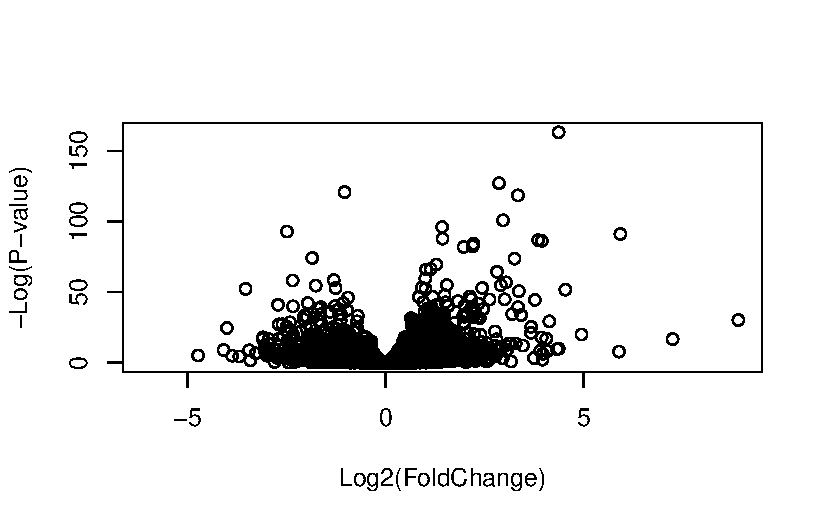
\includegraphics{Class12_files/figure-pdf/unnamed-chunk-25-1.pdf}

}

\end{figure}

\begin{Shaded}
\begin{Highlighting}[]
\FunctionTok{plot}\NormalTok{( res}\SpecialCharTok{$}\NormalTok{log2FoldChange,  }\SpecialCharTok{{-}}\FunctionTok{log}\NormalTok{(res}\SpecialCharTok{$}\NormalTok{padj), }
 \AttributeTok{ylab=}\StringTok{"{-}Log(P{-}value)"}\NormalTok{, }\AttributeTok{xlab=}\StringTok{"Log2(FoldChange)"}\NormalTok{)}

\CommentTok{\# Add some cut{-}off lines}
\FunctionTok{abline}\NormalTok{(}\AttributeTok{v=}\FunctionTok{c}\NormalTok{(}\SpecialCharTok{{-}}\DecValTok{2}\NormalTok{,}\DecValTok{2}\NormalTok{), }\AttributeTok{col=}\StringTok{"darkgray"}\NormalTok{, }\AttributeTok{lty=}\DecValTok{2}\NormalTok{)}
\FunctionTok{abline}\NormalTok{(}\AttributeTok{h=}\SpecialCharTok{{-}}\FunctionTok{log}\NormalTok{(}\FloatTok{0.05}\NormalTok{), }\AttributeTok{col=}\StringTok{"darkgray"}\NormalTok{, }\AttributeTok{lty=}\DecValTok{2}\NormalTok{)}
\end{Highlighting}
\end{Shaded}

\begin{figure}[H]

{\centering 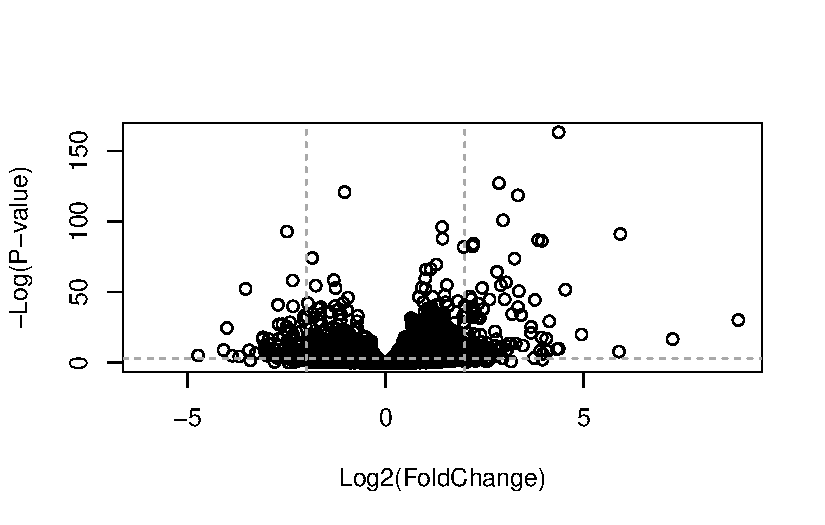
\includegraphics{Class12_files/figure-pdf/unnamed-chunk-26-1.pdf}

}

\end{figure}

\begin{Shaded}
\begin{Highlighting}[]
\CommentTok{\# Setup our custom point color vector }
\NormalTok{mycols }\OtherTok{\textless{}{-}} \FunctionTok{rep}\NormalTok{(}\StringTok{"gray"}\NormalTok{, }\FunctionTok{nrow}\NormalTok{(res))}
\NormalTok{mycols[ }\FunctionTok{abs}\NormalTok{(res}\SpecialCharTok{$}\NormalTok{log2FoldChange) }\SpecialCharTok{\textgreater{}} \DecValTok{2}\NormalTok{ ]  }\OtherTok{\textless{}{-}} \StringTok{"red"} 

\NormalTok{inds }\OtherTok{\textless{}{-}}\NormalTok{ (res}\SpecialCharTok{$}\NormalTok{padj }\SpecialCharTok{\textless{}} \FloatTok{0.01}\NormalTok{) }\SpecialCharTok{\&}\NormalTok{ (}\FunctionTok{abs}\NormalTok{(res}\SpecialCharTok{$}\NormalTok{log2FoldChange) }\SpecialCharTok{\textgreater{}} \DecValTok{2}\NormalTok{ )}
\NormalTok{mycols[ inds ] }\OtherTok{\textless{}{-}} \StringTok{"blue"}

\CommentTok{\# Volcano plot with custom colors }
\FunctionTok{plot}\NormalTok{( res}\SpecialCharTok{$}\NormalTok{log2FoldChange,  }\SpecialCharTok{{-}}\FunctionTok{log}\NormalTok{(res}\SpecialCharTok{$}\NormalTok{padj), }
 \AttributeTok{col=}\NormalTok{mycols, }\AttributeTok{ylab=}\StringTok{"{-}Log(P{-}value)"}\NormalTok{, }\AttributeTok{xlab=}\StringTok{"Log2(FoldChange)"}\NormalTok{ )}

\CommentTok{\# Cut{-}off lines}
\FunctionTok{abline}\NormalTok{(}\AttributeTok{v=}\FunctionTok{c}\NormalTok{(}\SpecialCharTok{{-}}\DecValTok{2}\NormalTok{,}\DecValTok{2}\NormalTok{), }\AttributeTok{col=}\StringTok{"gray"}\NormalTok{, }\AttributeTok{lty=}\DecValTok{2}\NormalTok{)}
\FunctionTok{abline}\NormalTok{(}\AttributeTok{h=}\SpecialCharTok{{-}}\FunctionTok{log}\NormalTok{(}\FloatTok{0.05}\NormalTok{), }\AttributeTok{col=}\StringTok{"gray"}\NormalTok{, }\AttributeTok{lty=}\DecValTok{2}\NormalTok{)}
\end{Highlighting}
\end{Shaded}

\begin{figure}[H]

{\centering 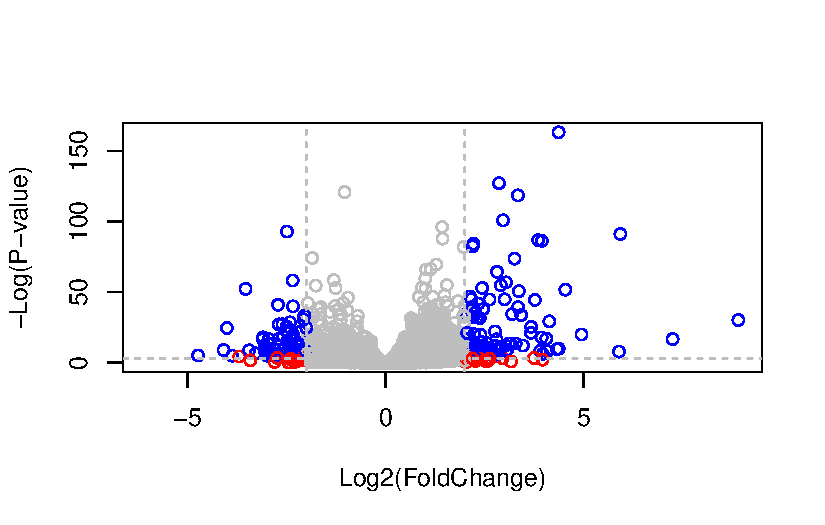
\includegraphics{Class12_files/figure-pdf/unnamed-chunk-27-1.pdf}

}

\end{figure}

\begin{Shaded}
\begin{Highlighting}[]
\FunctionTok{library}\NormalTok{(EnhancedVolcano)}
\end{Highlighting}
\end{Shaded}

\begin{verbatim}
Loading required package: ggplot2
\end{verbatim}

\begin{verbatim}
Loading required package: ggrepel
\end{verbatim}

\begin{Shaded}
\begin{Highlighting}[]
\NormalTok{x }\OtherTok{\textless{}{-}} \FunctionTok{as.data.frame}\NormalTok{(res)}

\FunctionTok{EnhancedVolcano}\NormalTok{(x,}
    \AttributeTok{lab =}\NormalTok{ x}\SpecialCharTok{$}\NormalTok{symbol,}
    \AttributeTok{x =} \StringTok{\textquotesingle{}log2FoldChange\textquotesingle{}}\NormalTok{,}
    \AttributeTok{y =} \StringTok{\textquotesingle{}pvalue\textquotesingle{}}\NormalTok{)}
\end{Highlighting}
\end{Shaded}

\begin{figure}[H]

{\centering 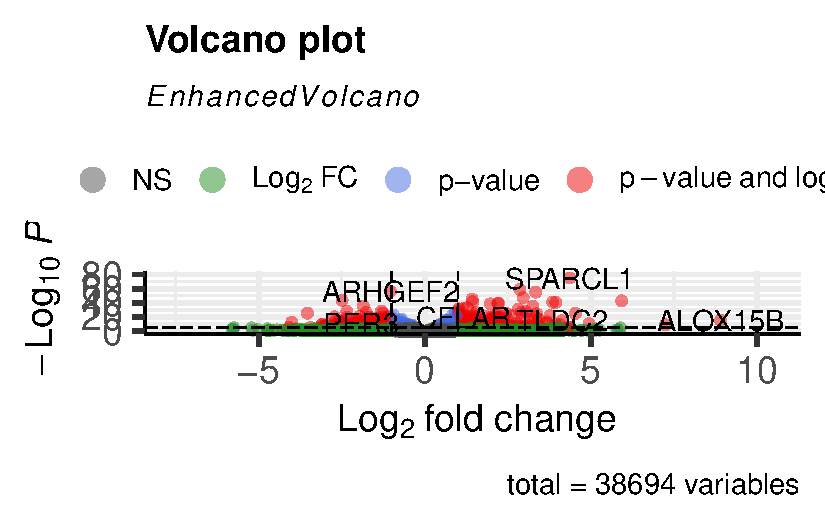
\includegraphics{Class12_files/figure-pdf/unnamed-chunk-28-1.pdf}

}

\end{figure}

\hypertarget{pathway-analysis}{%
\section{Pathway Analysis}\label{pathway-analysis}}

\begin{Shaded}
\begin{Highlighting}[]
\FunctionTok{library}\NormalTok{(pathview)}
\FunctionTok{library}\NormalTok{(gage)}
\FunctionTok{library}\NormalTok{(gageData)}

\FunctionTok{data}\NormalTok{(kegg.sets.hs)}

\CommentTok{\# Examine the first 2 pathways in this kegg set for humans}
\FunctionTok{head}\NormalTok{(kegg.sets.hs, }\DecValTok{2}\NormalTok{)}
\end{Highlighting}
\end{Shaded}

\begin{verbatim}
$`hsa00232 Caffeine metabolism`
[1] "10"   "1544" "1548" "1549" "1553" "7498" "9"   

$`hsa00983 Drug metabolism - other enzymes`
 [1] "10"     "1066"   "10720"  "10941"  "151531" "1548"   "1549"   "1551"  
 [9] "1553"   "1576"   "1577"   "1806"   "1807"   "1890"   "221223" "2990"  
[17] "3251"   "3614"   "3615"   "3704"   "51733"  "54490"  "54575"  "54576" 
[25] "54577"  "54578"  "54579"  "54600"  "54657"  "54658"  "54659"  "54963" 
[33] "574537" "64816"  "7083"   "7084"   "7172"   "7363"   "7364"   "7365"  
[41] "7366"   "7367"   "7371"   "7372"   "7378"   "7498"   "79799"  "83549" 
[49] "8824"   "8833"   "9"      "978"   
\end{verbatim}

\begin{Shaded}
\begin{Highlighting}[]
\NormalTok{foldchanges }\OtherTok{=}\NormalTok{ res}\SpecialCharTok{$}\NormalTok{log2FoldChange}
\FunctionTok{names}\NormalTok{(foldchanges) }\OtherTok{=}\NormalTok{ res}\SpecialCharTok{$}\NormalTok{entrez}
\FunctionTok{head}\NormalTok{(foldchanges)}
\end{Highlighting}
\end{Shaded}

\begin{verbatim}
       7105       64102        8813       57147       55732        2268 
-0.35070302          NA  0.20610777  0.02452695 -0.14714205 -1.73228897 
\end{verbatim}

\begin{Shaded}
\begin{Highlighting}[]
\CommentTok{\# Get the Results}
\NormalTok{keggres }\OtherTok{=} \FunctionTok{gage}\NormalTok{(foldchanges, }\AttributeTok{gsets=}\NormalTok{kegg.sets.hs)}
\FunctionTok{attributes}\NormalTok{(keggres)}
\end{Highlighting}
\end{Shaded}

\begin{verbatim}
$names
[1] "greater" "less"    "stats"  
\end{verbatim}

\begin{Shaded}
\begin{Highlighting}[]
\CommentTok{\# Look at the first three down (less) pathways}
\FunctionTok{head}\NormalTok{(keggres}\SpecialCharTok{$}\NormalTok{less, }\DecValTok{3}\NormalTok{)}
\end{Highlighting}
\end{Shaded}

\begin{verbatim}
                                      p.geomean stat.mean        p.val
hsa05332 Graft-versus-host disease 0.0004250461 -3.473346 0.0004250461
hsa04940 Type I diabetes mellitus  0.0017820293 -3.002352 0.0017820293
hsa05310 Asthma                    0.0020045888 -3.009050 0.0020045888
                                        q.val set.size         exp1
hsa05332 Graft-versus-host disease 0.09053483       40 0.0004250461
hsa04940 Type I diabetes mellitus  0.14232581       42 0.0017820293
hsa05310 Asthma                    0.14232581       29 0.0020045888
\end{verbatim}

\begin{Shaded}
\begin{Highlighting}[]
\FunctionTok{pathview}\NormalTok{(}\AttributeTok{gene.data=}\NormalTok{foldchanges, }\AttributeTok{pathway.id=}\StringTok{"hsa05310"}\NormalTok{)}
\end{Highlighting}
\end{Shaded}

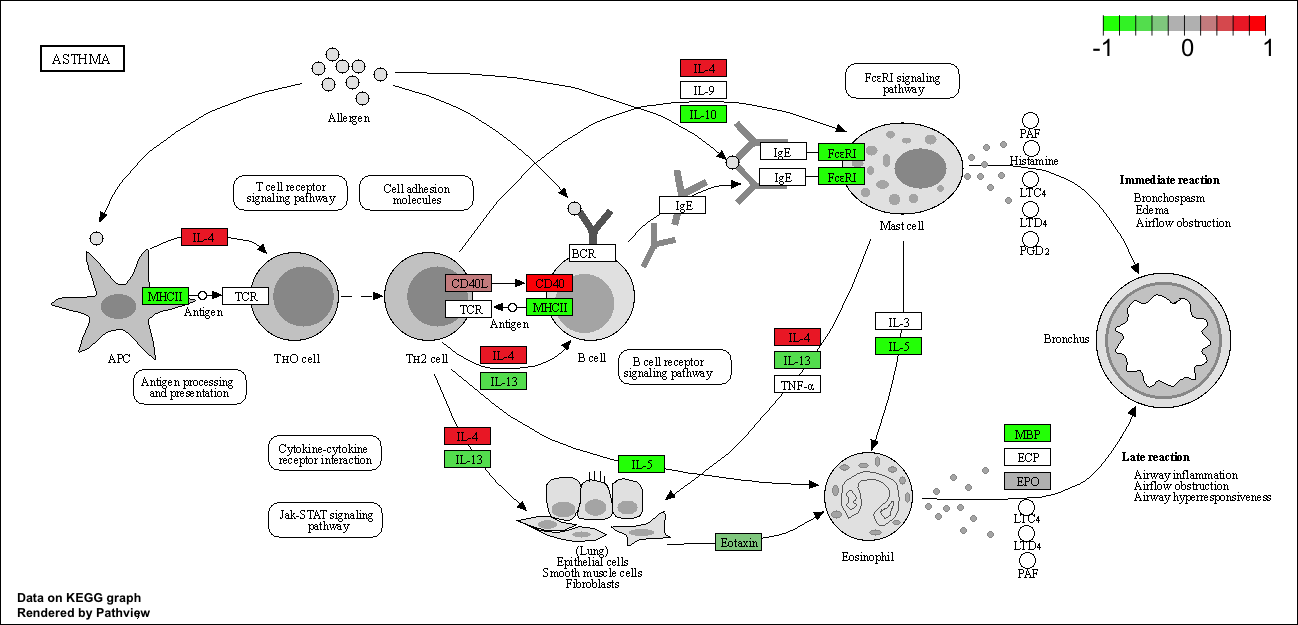
\includegraphics{hsa05310.pathview.png}

\begin{Shaded}
\begin{Highlighting}[]
\CommentTok{\# A different PDF based output of the same data}
\FunctionTok{pathview}\NormalTok{(}\AttributeTok{gene.data=}\NormalTok{foldchanges, }\AttributeTok{pathway.id=}\StringTok{"hsa05310"}\NormalTok{, }\AttributeTok{kegg.native=}\ConstantTok{FALSE}\NormalTok{)}
\end{Highlighting}
\end{Shaded}




\end{document}
